\section{Visualisierung}
\label{sec:DesktopApp}
Diese Sektion beschreibt die Bedienung und Funktionsweise der eigens entwickelten Desktopanwendung, welche zur einfachen Visualisierung und Auswertung der Daten dient.
\subsection{Grundlagen}
\label{subsec:VisGrundlagen}
Für die Programmierung der Desktopanwendung wird ebenfalls Python verwendet, in diesem Fall wird zusätzlich auch Qt verwendet. Qt ist, wie in Sektion \ref{subsubsec:tQt} beschreiben, eine Bibliothek zur Entwicklung von grafischen Oberflächen, was eine Erleichterung in der Entwicklung von Desktopanwendungen darstellt. Die Desktopanwendung dieser Diplomarbeit ist in vier Ansichten aufgeteilt. Wird das Programm gestartet, wird zunächst die \glqq Overview\grqq angezeigt. In dieser Ansicht sind ein \ac{3D}-Modell des Autos und drei Schaltflächen zu sehen. Die Schaltflächen führen zu den anderen Ansichten, darunter die \glqq Table View\grqq , die \glqq Plot View\grqq \ und die \glqq Map View\grqq .
\subsection{Table View}
\label{subsec:VisTableView}
Eine weitere Ansicht ist, wie bereits erwähnt, die \glqq Table View\grqq , in welcher eine Tabelle mit allen Messwerten der geöffneten Datei zu sehen ist. In der Table View sind wie in Abbildung \ref{fig:TableView} abgebildet am oberen Rand der Tabelle Identifikatoren zu sehen, welche die Aufgabe haben, die Werte realen Größen zuordenbar zu machen.
\begin{figure}[h]
\centering
\missingfigure{}
\caption{Table View}
\label{fig:TableView}
\end{figure}
\\
Die Tabelle wird mithilfe des Qt-Widgets \glqq QTableWidget\grqq erstellt und angezeigt. Dazu werden die Zeiten als Beschriftungen der Zeilen und die Namen der Messwerte als Beschriftung der Spalten verwendet. 

\subsection{Plot View}
\label{subsec:VisPlotView}
Da eine Tabelle unübersichtlich sein kann und Menschen reine Zahlenwerte oft nicht mit Fahrverhältnissen in Verbindung bringen können, gibt es auch die \glqq Plot View\grqq . In dieser Ansicht werden alle Werte in einem Graphen gezeichnet.
\subsubsection{Funktionen der Plot View}
\label{subsubsec:PlotViewFunktion}
Nach dem Einlesen der Daten ordnet das Programm alle Messwerte standardmäßig der 1. Ordinate zu. Die Benutzeroberfläche hat aber die Fähigkeit, auf bis zu drei verschiedenen Ordinaten zu plotten. Diese Ordinaten sind immer alle derselben Abszisse zugeordnet, die einen Zeitverlauf darstellt. Alle Achsen sind dynamisch, bei einer Vergrößerung der Ansicht ändern sich alle Achsenbeschriftungen somit im selben Verhältnis wie die Messwerte. Da das Auftragen von verschiedenen Einheiten auf derselben Achse in einigen Fällen zu unübersichtlichen und falsch skalierten Ansichten führen kann, können die aufgenommenen Werte in den Einstellungen der Software auf andere Achsen gelegt werden. Das Einstellungsfenster ist in Abbildung \ref{fig:plotsettings} zu sehen.
\begin{figure}[h]
\centering
\missingfigure{}
\caption{Plot-Einstellungen}
\label{fig:plotsettings}
\end{figure}
\\
Eine weitere Funktion dieser Ansicht ist das optional aktivierbare Gitter, das das Zuweisen von im Graphen angezeigten Werten zu den an den Achsen angezeigten Zahlen vereinfacht. Dieses Gitter kann in einem per \glqq Rechtsklick\grqq \ aufrufbaren Kontextmenü aktiviert werden. Ein Bildschirmausschnitt der \glqq Plot View\grqq \ mit beispielhaften Einstellungen und Werten ist in Abbildung \ref{fig:PlotView} ersichtlich. Die Legende, die in Abbildung \ref{fig:PlotView} links oben zu sehen ist, hat den Auftrag, die Farben den Messwerten zuordenbar zu machen. Wenn ein Element der Legende angeklickt wird, wird die Sichtbarkeit des Elements umgeschaltet. Somit können einzelne Werte einfach ein- und ausgeblendet werden.
\begin{figure}[h]
\centering
\missingfigure{}
\caption{Plot View}
\label{fig:PlotView}
\end{figure}
\\
Außerdem kann in dem mit einem \glqq Rechtsklick\grqq \ aufrufbaren Kontextmenü die aktuelle Ansicht exportiert werden. Als Exportformat stehen dabei \glqq Bilddatei\grqq ,\ \glqq \ac{SVG}\grqq , \glqq Matplotlib-Fenster\grqq\ und \glqq \ac{CSV}\grqq\ zur Verfügung. Unter \glqq Bilddatei\grqq\ fallen in diesem Fall die Formate \glqq\ac{PNG}\grqq , \glqq\ac{TIF}\grqq\ und \glqq\ac{JPG}- Datei\grqq .
\subsubsection{Implementation der Plot View}
\label{subsubsec:PlotViewImplementation}
Die \grqq\ Plot View \glqq wird mithilfe der in Sektion \ref{subsubsec:tPyQtGraph} Python-Bibliothek \glqq PyQtGraph\grqq \ gezeichnet. Dazu werden zunächst die Zeitstempel aus dem Datenfile den Zeitwerten der Abszisse zugeordnet. Anschließend werden alle Datensets, die Fehler enthalten aus dem Datenpool entfernt. Ist dies geschehen, werden die Achsenbeschriftungen, welche in den Plot-Einstellungen eingestellt wurden, zu den jeweiligen Achsen zugeordnet und der Graph initialisiert. Beim Initialisieren des Graphen werden die Werte in den Graphen eingezeichnet und den jeweiligen Achsen zugeordnet. Sollten Einstellungen im Einstellungsfenster geändert werden, wird dieser Prozess erneut durchgeführt, um den Graph an die neue Achsbelegung anzupassen.
\subsection{Map View}
\label{subsec:VisMapView}
Die \glqq Map View\grqq\ hat die Aufgabe, dem Nutzer eine grafische Darstellung der aufgezeichneten \ac{GPS}-Koordinaten zu bieten. Für diese Darstellung wird eine aktive Internetverbindung benötigt, um die Karte herunterzuladen.
\subsubsection{Funktionen der Map View}
\label{subsubsec:MapViewFunktion}
Um die Werte darzustellen, werden alle Längen- und Breitengrade aus der geöffneten Datei extrahiert, dynamisch die benötigten \ac{OSM} Tiles aus dem Internet heruntergeladen und anschließend ein Pfad aus den Koordinaten auf die Karte gezeichnet. Ein Beispiel für eine solche Karte ist in Abbildung 
\ref{fig:OSMMapView} zu sehen. Wenn das Bedürfnis besteht, die Karte für das Verwenden an einem späteren Zeitpunkt abzuspeichern, kann dies mit einem Klick auf den Knopf \glqq Save Image\grqq\ getan werden. Somit wird ein Dialogfenster zur Auswahl des Speicherortes geöffnet und anschließend wird die Karte als \ac{SVG} am gewählten Ort abgespeichert.
\begin{figure}[h]
\centering
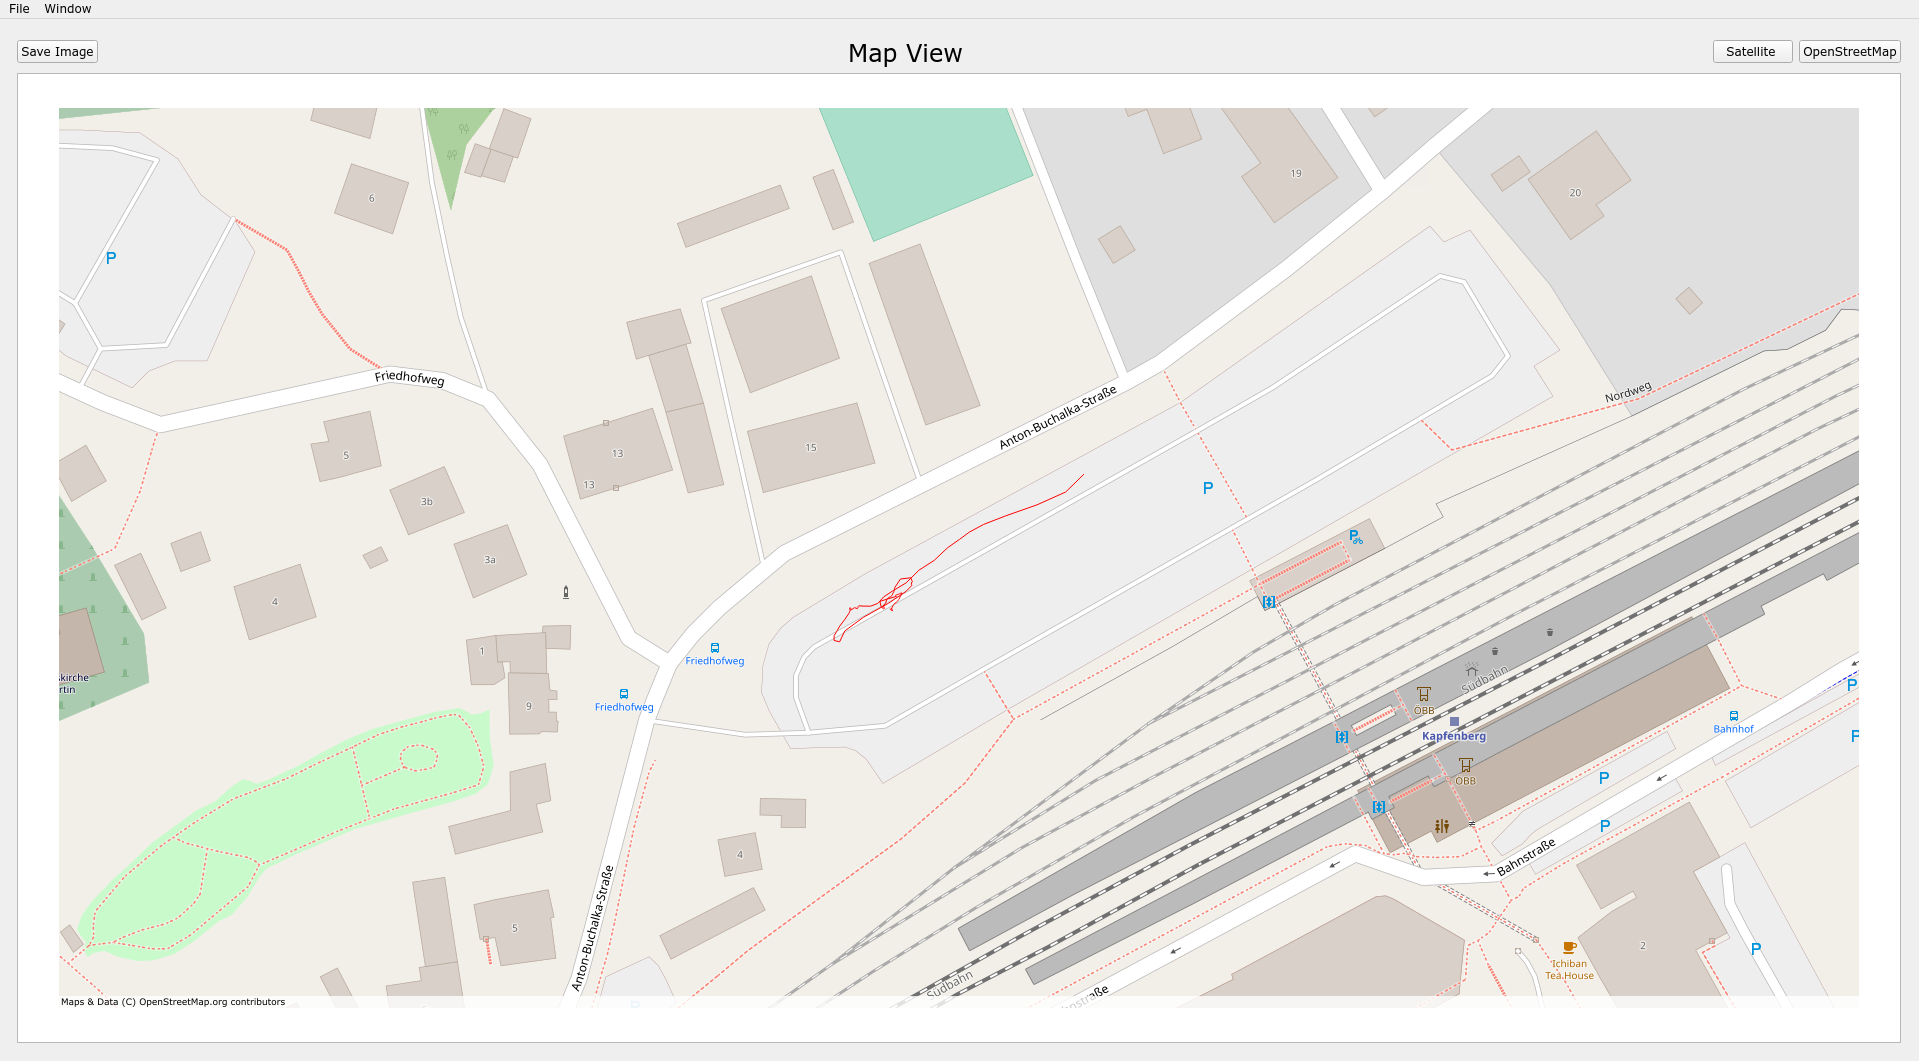
\includegraphics[scale=0.295]{MapViewOSM.png}
\caption{Map View - \ac{OSM}}
\label{fig:OSMMapView}
\end{figure}
\\
Dieselbe Ansicht ist auch als Satellitenbild verfügbar, die Vorgehensweise ist hierbei beinahe ident, anstelle von \ac{OSM} werden die Tiles in diesem Fall von \glqq ArcGISWorldImagery\grqq\ bezogen. Eine solche Karte, ist in Abbildung \ref{fig:SatteliteMapView} ersichtlich. 
\begin{figure}[h]
\centering
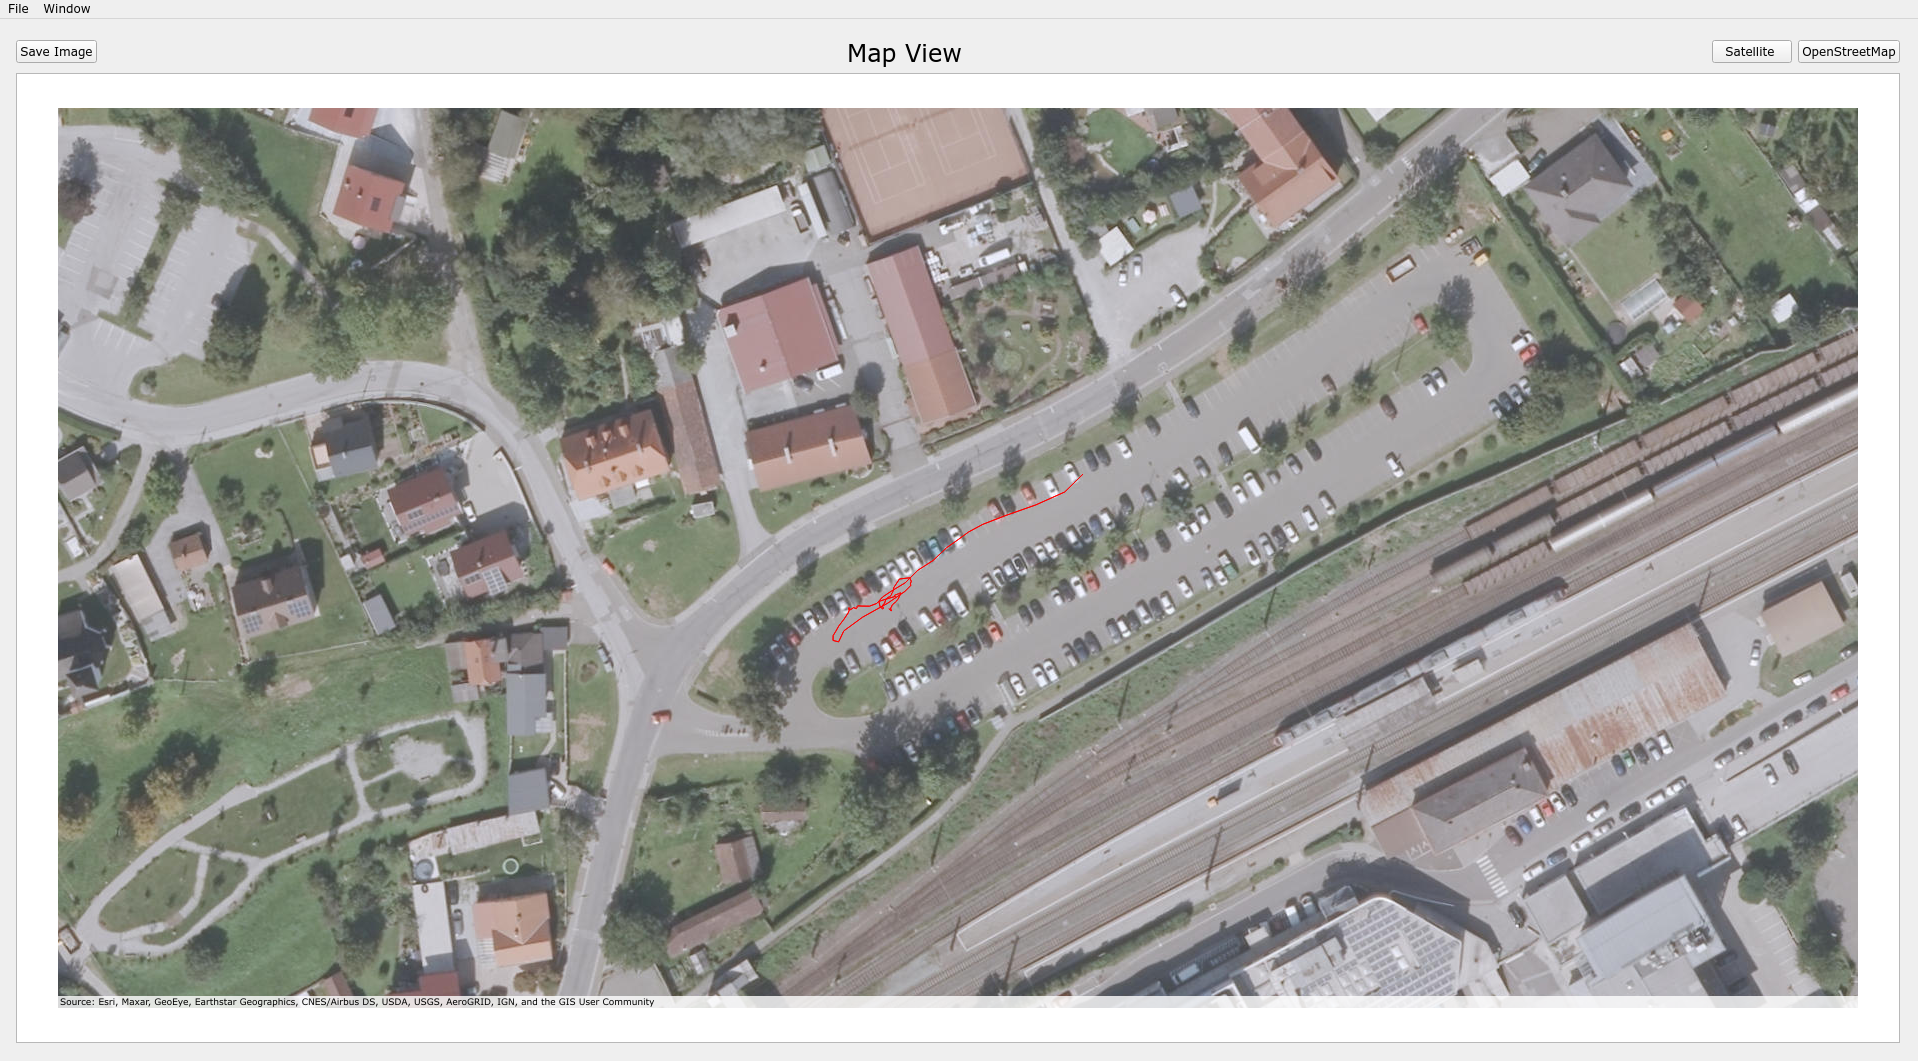
\includegraphics[scale=0.295]{MapViewSatellit.png}
\caption{Map View - Satellitenbild}
\label{fig:SatteliteMapView}
\end{figure}

\subsubsection{Implementation der Map View}
\label{subsubsec:MapViewImplementation}
Diese Ansicht wird mithilfe der in Sektion \ref{subsubsec:tStaticmaps} Python-Bibliothek \glqq py-staticmaps\grqq \ realisiert. Zunächst werden die Koordinaten aus dem Datenset extrahiert, dann werden die einzelnen Punkte miteinander verbunden, um einen Pfad darzustellen. Um den Kartenteil, der heruntergeladen werden soll, festzustellen, wird das Zentrum des Pfades errechnet. Da die Reichweite des ferngesteuerten Autos durch die Sichtweite des Fahrers limitiert ist, kann immer der \ac{OSM}-Zoomfaktor 19 für die Karte verwendet werden. Dieses Kartenstück wird von OpenStreetMap heruntergeladen und mithilfe des Qt-Widgets \glqq QGraphicsView\grqq\ angezeigt.